%%%%%%%%%%%%%%%%%%%%%%%%%%%%%%%%%%%%%%%%%%%%%%%%%%%%%%%%%%%%%%%%%%%%%%%%%%
\chapter{Bajtkód jazyka Java}\label{Bytecode}

Architektura Javy se podle Vennerse \cite{Venners:InsideJVM} skládá z~programovacího jazyka Java, formátu instrukčního souboru, aplikačního programového rozhraní Java Application Programming Interface (Java API) a virtuálního stroje Java Virtual Machine (JVM). Pro psaní zdrojových kódů a jejich spouštění je zapotřebí všech těchto částí.
Zdrojový kód zapsaný v~programovacím jazyce Java je uložený v~souboru s~příponou \texttt{.java} (dále \texttt{java} souboru). Tento kód je při kompilaci převeden na mezikód, tzv. bajtkód, a uložen v~souborech s~příponou \texttt{.class} (dále \texttt{class} souborech). Bajtkód lze následně spustit pomocí virtuálního stroje, který má přístup k~Java API. 
V~této kapitole popisuji základní charakteristiky JVM a formát jeho instrukčního souboru dle specifikace ve verzi Java SE 8 Edition \cite{Lindholm:JVM}.

%%%%%%%%%%%%%%%%%%%%%%%%%%%%%%%%%%%%%%%%%%%%%%%%%%%%%%%%%%%%%%%%%%%%%%%%%%
\section{Virtuální stroj JVM}\label{Bytecode:JVM}

O~JVM lze  hovořit z~hlediska abstraktní specifikace nebo konkrétní implementace. Konkrétní implementace je závislá na daném systému a hardwaru, ale jednotná interpretace \texttt{class} souborů napříč platformami je zajištěna dodržením specifikace a platformově nezávislým formátem \texttt{class} souborů. Vzhledem k~zaměření práce se v~této kapitole zabývám abstraktní specifikací JVM.

\subsection{Datové typy a hodnoty}

Datové typy a hodnoty podporované JVM jsou znázorněné na obrázku \ref{fig:types}. Celá čísla jsou reprezentovaná datovými typy \texttt{byte} o~šířce 8 bitů, \texttt{short} o~šířce 16 bitů, \texttt{int} o~šířce 32 bitů nebo \texttt{long} o~šířce 64 bitů. Pro čísla s~plovoucí řádovou čárkou jsou definovány typy \texttt{float} o~32 bitech a \texttt{double} o~64 bitech. Typ \texttt{boolean} reprezentuje pravdivostní hodnoty pravda a nepravda. Typ \texttt{returnAddress} reprezentuje ukazatel na instrukci v~instrukčním souboru.

Znaky a řetězce jsou v~Javě kódované podle standardu Unicode v~kódování UTF-16, kde jeden znak je kódovaný jednou nebo dvěma kódovými jednotkami. Kódovou jednotku reprezentuje typ \texttt{char}. Jedná se o~16-bitové nezáporné číslo. Řetězec je pak reprezentovaný pomocí pole hodnot typu \texttt{char}. V~instrukčním souboru jsou řetězcové konstanty kódované v~modifikovaném kódování UTF-8. 

Typ \texttt{reference} označuje referenční datový typ a reprezentuje referenci na dynamicky vytvořený objekt. Podle toho, zda objekt je instancí třídy, pole nebo instancí třídy či pole, které implementují nějaké rozhraní, se rozlišuje typ reference. Hodnotou typu \texttt{reference} může být též speciální hodnota \texttt{null}, tedy reference na žádný objekt. 

\begin{figure}[!h]
\centering
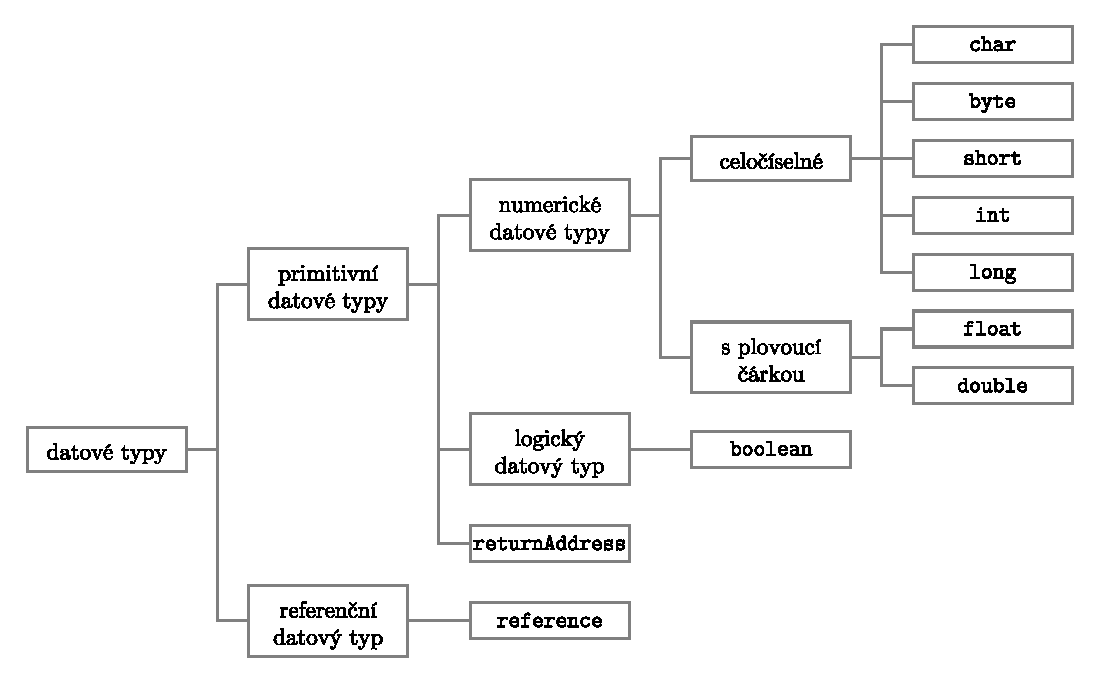
\includegraphics[scale=0.8]{fig/types}
\caption{Datové typy a hodnoty podporované JVM.}\label{fig:types}
\end{figure}

Instrukční sada JVM je omezená a nenabízí u~všech instrukcí podporu pro všechny datové typy. Celá čísla jsou primárně reprezentovaná datovými typy \texttt{int} a \texttt{long} a případně přetypovaná na jeden z~typů \texttt{byte}, \texttt{short} či \texttt{char}. Pro datový typ \texttt{boolean} existuje jen podpora pro přetypování a pro vytvoření pole hodnot typu \texttt{boolean}. Pro výpočet logických výrazů se používá typ \texttt{int} s~hodnotami 0 a 1.


\subsection{Paměťové oblasti}

JVM pracuje s~několika typy paměťových oblastí. Velikosti těchto oblastí mohou být pevně dané, nebo se mohou měnit dynamicky podle potřeby. Při spuštění JVM vzniká halda a oblast metod. Halda je paměť určená pro alokaci instancí tříd a polí. Alokovanou paměť nelze dealokovat explicitně. Haldu automaticky spravuje tzv. \textit{garbage collector}. Oblast metod slouží k~ukládání kompilovaného kódu. Pro každou načtenou třídu se do této paměti ukládají struktury definující tuto třídu. Jednou z~těchto struktur je tzv. \textit{run-time constant pool}. Jedná se o~tabulku konstant z~\texttt{class} souboru, v~níž jsou symbolické reference na třídy, metody a členské proměnné nahrazeny konkrétními referencemi. Více se o~tabulce konstant zmiňuje kapitola \ref{Bytecode:Format:Constants}.

Každá aplikace je spuštěna v~samostatném vlákně a při běhu mohou vznikat a zanikat i další vlákna. Všechna taková vlákna sdílí přístup k~haldě a oblasti metod. Navíc má každé vlákno k~dispozici vlastní \texttt{pc} registr a zásobník rámců. V~\texttt{pc} registru je uchováván ukazatel na aktuálně vykonávanou instrukci, není-li aktuálně vykonávaná metoda nativní. Zásobník rámců obsahuje data zavolaných metod. Při každém volání metody je vytvořen nový rámec. Rámec má vlastní pole lokálních proměnných a zásobník operandů. V~poli lokálních proměnných se uchovávají hodnoty parametrů a lokálních proměnných. Hodnoty lze vkládat na zásobník operandů, provádět nad nimi výpočty a ukládat zpět do pole. Operační zásobník slouží k~předávání operandů instrukcím a k~uchovávání mezivýsledků. Podílí se také na předávání parametrů a návratových hodnot volaných metod.

Před voláním metody je třeba nejprve vložit parametry na zásobník operandů aktuálního rámce. Zavoláním metody se vytvoří nový rámec a umístí se na vrchol zásobníku rámců. Parametry se následně přesunou ze zásobníku operandů předchozího rámce do pole lokálních proměnných nového rámce. Registr \texttt{pc} se nastaví na první instrukci volané metody a začnou se vykonávat jednotlivé instrukce. Při návratu z~metody je návratová hodnota umístěná na vrcholu zásobníku operandů, vrací-li metoda nějakou hodnotu. Tato hodnota je přesunuta na zásobník operandů předcházejícího rámce a aktuální rámec je ze zásobníku rámců odstraněn. Dojde k~obnovení stavu volající metody. Registr \texttt{pc} je nastaven na index instrukce, která bezprostředně následuje za instrukcí volající metodu. Pokud je metoda ukončena vyvoláním nezachycené výjimky, pak k~předání hodnoty nedochází. Aktuální rámec je odstraněn a výjimka je znovu vyvolaná ve volající metodě. Zpracování výjimek je více vysvětleno v~kapitole \ref{Bytecode:Format:Method}.

Nejmenším prvkem, se kterým pracuje zásobník operandů, je 32-bitová hodnota. Hodnoty většiny datových typů lze vyjádřit pomocí jediného prvku, ale hodnoty typů \texttt{long} a \texttt{double} je třeba reprezentovat dvěma prvky. S~takovou dvojicí je třeba vždy manipulovat jako s~celkem. Datový typ hodnoty na zásobníku je daný instrukcí, která ho tam vložila, a na hodnotu nelze nahlížet jinak. Hloubka zásobníku operandů je určená počtem prvků na zásobníku. Lze tedy definovat pojem jednotka hloubky zásobníku, kdy jedna jednotka odpovídá jednomu prvku za zásobníku.

Lokální proměnná v~poli lokálních proměnných je 32-bitová hodnota. Proměnnou lze adresovat pomocí indexu do pole, kde pole je indexováno od nuly. Lokální proměnná může být typu \texttt{byte}, \texttt{short}, \texttt{int}, \texttt{char}, \texttt{float}, \texttt{boolean}, \texttt{reference} nebo \texttt{returnAddress}. Hodnoty typu \texttt{long} a \texttt{double} jsou uchovávané pomocí dvojice lokálních proměnných. V~tom případě k~adresaci slouží nižší z~indexů a na větší index se nesmí přistupovat. 


\subsection{Kontrola instrukčního souboru}

Při načítání \texttt{class} souboru je ověřeno správné formátování tak, jak je popsáno v~kapitole \ref{Bytecode:Format}. Jsou zkontrolovány první čtyři bajty souboru, předdefinované atributy musí být správné délky, názvy a typy tříd, rozhraní, metod a proměnných musí být validní, indexy do tabulky konstant musí adresovat správný typ položky. Dále jsou kladena jistá omezení na kód metod. Mimo jiné, argumenty instrukcí musí mít správný typ a musí být správného počtu, integrita hodnot typu \texttt{long} a \texttt{double} nemůže být nikdy narušena, k~hodnotě lokální proměnné se nesmí přistupovat před inicializací proměnné a nesmí dojít k~načtení hodnoty z~prázdného zásobníku operandů, či překročení jeho maximální velikosti. Metody musí být ukončené některou z~instrukcí pro návrat z~metody. Součástí verifikace těchto omezení je typová kontrola nebo typová inference. Díky kontrole instrukčního souboru se omezení nemusí kontrolovat za běhu programu.

%=========================================================================

%%%%%%%%%%%%%%%%%%%%%%%%%%%%%%%%%%%%%%%%%%%%%%%%%%%%%%%%%%%%%%%%%%%%%%%%%%
\section{Formát instrukčního souboru}\label{Bytecode:Format}

% doplnit příklady

Při kompilaci \texttt{java} souboru překladač pro každou definovanou třídu a rozhraní vytvoří jeden \texttt{class} soubor. Tento soubor obsahuje binární reprezentaci kompilovaného mezikódu, který lze interpretovat prostřednictvím JVM.  Tato kapitola je věnovaná popisu formátu \texttt{class} souboru.

Pro popis formátu jsem zvolila rozšířenou Backus-Naurovu formu, která umožňuje zapsat syntaxi formálního jazyka pomocí pravidel a terminálních a nonterminálních symbolů. Nonterminální symboly jsou definovány pomocí definujícího symbolu \texttt{:=}, symbolu pro konkatenaci \texttt{,}, symbolu pro alternaci \texttt{$\mathtt{|}$}, symbolů pro nula a více opakování \texttt{\{\}}, ukončujícího symbolu \texttt{;} a pomocí graficky odlišených \T{terminálních} a \N{nonterminálních} symbolů. Symboly popisují jednotlivé struktury, ze kterých se \texttt{class} soubor skládá.

\subsection{Základní struktura}\label{Bytecode:Format:Basic}

Položky \texttt{class} souboru tvoří posloupnost bajtů. Základní stavební jednotkou je tedy bajt, který je v~pravidlech reprezentovaný symbolem \N{B}. Symbol $\langle n \rangle$\N{B}, kde $\langle n \rangle \in \{2,3,\dots\}$, reprezentuje $n$ bajtů. Terminály začínají prefixem \texttt{0x} a jsou hexadecimální reprezentací posloupnosti bajtů. 

Základní struktura souboru je popsaná symbolem \N{classfile}. Soubor obsahuje informace o~svém typu a verzi (\N{version}), disponuje tabulkou všech konstant, které se v~souboru vyskytují (\N{constants}), nese informace o~třídě či rozhraní (\N{class}), které reprezentuje, obsahuje seznam rozhraní (\N{interface\_list}), které reprezentovaná třída implementuje, případně rozhraní rozšiřuje, seznam členských proměnných (\N{field\_list}), seznam metod (\N{method\_list}) a seznam atributů (\N{attribute\_list}). 

\begin{figure}[h!]
  \begin{tabular}{r c l}
  \N{classfile} &:=& \N{version}, \N{constants}, \N{class}, \N{interface\_list}, \N{field\_list}, \N{method\_list}, \N{attribute\_list};
  \end{tabular}
\end{figure}

Typ souboru je definován prvními čtyřmi bajty, které jsou popsané symbolem \N{magic\_number}. Verze souboru je tvořena hodnotou $M$ symbolu \N{major\_version} a hodnotou $m$ symbolu \N{minor\_version} jako $M.m$.

\begin{figure} [h!]
  \begin{tabular}{r c l}
  \N{version} &:=& \N{magic\_number}, \N{minor\_version}, \N{major\_version};\\
  \N{magic\_number} &:=& \T{0xCAFEBABE};\\
  \N{minor\_version} &:=& \N{2B};\\
  \N{major\_version} &:=& \N{2B};\\
  \end{tabular}
\end{figure}

\subsection{Konstanty}\label{Bytecode:Format:Constants}

Tabulka konstant obsahuje některé číselné konstanty, všechny řetězce a symbolické informace o~všech třídách, rozhraních, metodách a členských proměnných, které se v~souboru, instrukcích i atributech vyskytují. Tato tabulka se nazývá \textit{constant pool} a slouží v~podstatě jako databáze dat, do které se pomocí indexů odkazují další položky souboru. Odkazem do tabulky konstant je tedy v~dalším textu myšlen platný index do tabulky konstant adresující položku očekávaného typu.

Struktura tabulky konstant je popsána symbolem \N{constants}. Symbol \N{constant\_pool\_count} reprezentuje hodnotu $1 + n$, kde $n$ je počet položek v~tabulce konstant. Položky tabulky jsou indexované od jedné, neboť nultý index je vyhrazen pro odkaz na žádnou z~položek. Samotná tabulka je reprezentovaná symbolem \N{constant\_pool}.

\begin{figure} [h!]

  \begin{tabular}{r c l}
  \N{constants} &:=& \N{constant\_pool\_count}, \N{constant\_pool}; \\
  \N{constant\_pool\_count} &:=& \N{2B}; \\
  \N{constant\_pool} &:=& \{
          \N{constant\_integer} \\
  &&  $|$ \N{constant\_float} \\
  &&  $|$ \N{constant\_long} \\
  &&  $|$ \N{constant\_double} \\ 
  &&  $|$ \N{constant\_utf8} \\
  &&  $|$ \N{constant\_string} \\ 
  &&  $|$ \N{constant\_nameAndType} \\ 
  &&  $|$ \N{constant\_class} \\
  &&  $|$ \N{constant\_fieldref} \\
  &&  $|$ \N{constant\_methodref} \\
  &&  $|$ \N{constant\_interfaceMethodref} \\
  &&  $|$ \N{constant\_methodHandle} \\ 
  &&  $|$ \N{constant\_methodType} \\
  &&  $|$ \N{constant\_invokeDynamic} \\ 
  &&  \}; \\
  \end{tabular}
\end{figure}

Každá položka tabulky je tvořena označením typu a posloupností bajtů s~informacemi o~položce. Položky mohou mít různou velikost v~závislosti na svém typu a obsahu. Stejným způsobem jsou definovány všechny tabulky v~\texttt{class} souboru. Jestliže se jedná o~pole, pak prvky pole jsou stejného typu, a proto označení typu v~prvcích chybí.

 Číselné konstanty jsou reprezentované symboly \N{constant\_integer}, \N{constant\_float}, \N{constant\_long} a \N{constant\_double} a skládají se jen z~typu a číselné hodnoty. 
Symbol \N{constant\_utf8} reprezentuje řetězec v~upraveném kódování \texttt{UTF-8} a skládá se z~typu, délky pole bajtů a pole bajtů nesoucích reprezentaci řetězce. Znaky řetězce mohou být vzhledem ke kódování tvořeny různými počty bajtů. 
Symbol \N{constant\_string} je reprezentací řetězcové konstanty a kromě typu obsahuje index do tabulky konstant na položku \N{constant\_utf8}. 
Třídy a rozhraní jsou reprezentované položkami \N{constant\_class} s~odkazy na jejich název (\N{constant\_utf8}). 
Entity jako členské proměnné (i statické), metody třídy a metody rozhraní jsou reprezentované položkami \N{constant\_fieldref}, \N{constant\_methodref} a \N{constant\_interfaceMethodref} obsahujícími odkaz na třídu, případně rozhraní, dané entity (\N{constant\_class}), a odkaz na položku se jménem a typem této entity (\N{constant\_nameAndType}). 
Jméno a typ v~položce \N{constant\_nameAndType} jsou odkazy na řetězce (\N{constant\_utf8}). 
Položky \N{constant\_methodHandle}, \N{constant\_methodType} a \N{constant\_invokeDynamic} souvisí s~podporou dynamických jazyků.


Názvy tříd a rozhraní jsou interně uváděné v~úplném tvaru, ale z~historických důvodů se tečky nahrazují lomítky. Například, třída \texttt{Object} má úplný název \texttt{java.lang.Object} a interní název \texttt{java/lang/Object}. Typ proměnné nebo metody je specifikován řetězcem. Základní datové typy jsou reprezentované písmeny \texttt{B} pro \texttt{byte}, \texttt{C} pro \texttt{char}, \texttt{D} pro \texttt{double}, \texttt{F} pro \texttt{float}, \texttt{I} pro \texttt{int}, \texttt{J} pro \texttt{long}, \texttt{S} pro \texttt{short}, \texttt{Z} pro \texttt{boolean}. Typ reference na objekt je reprezentovaný řetězcem \texttt{L}$ClassName$\texttt{;}, kde $ClassName$ je interní název třídy nebo rozhraní. Typ reference na jednorozměrné pole je reprezentovaný řetězcem \texttt{[}$ComponentType$, kde $ComponentType$ je řetězec reprezentující základní datový typ, referenci na objekt nebo referenci na pole. Pomocí zanoření referencí na pole lze definovat referenci na vícerozměrné pole. Například, řetězec \texttt{Ljava/lang/Object;} označuje referenci na objekt typu \texttt{Object} a \texttt{[[[I} označuje referenci na trojrozměrné pole typu \texttt{int}. Typ metody je reprezentován řetězcem, který se skládá z~výčtu typů formálních parametrů metody a typu její návratové hodnoty. Tedy například, typ metody s~hlavičkou \texttt{int method(boolean b, Object o)} bude specifikovaný řetězcem \texttt{(BLjava/lang/Object;)I}. Nemá-li metoda žádné parametry či nevrací žádnou hodnotu, pak je chybějící typ nahrazen písmenem \texttt{V}.


\subsection{Třída}\label{Bytecode:Format:Class}

Každý \texttt{class} soubor reprezentuje jednu třídu nebo rozhraní. Informace o~reprezentované entitě jsou definované symbolem \N{class}. Položka \N{this\_class} je odkazem na tuto entitu v~tabulce konstant, \N{super\_class} je odkaz na nadřazenou třídu a \N{access\_flags} je bitové pole příznaků pro přístup k~této entitě.

\begin{figure} [h!]
  \begin{tabular}{r c l}
  \N{class} &:=& \N{access\_flags}, \N{this\_class}, \N{super\_class};\\
  \N{access\_flags} &:=& \N{2B}; \\
  \N{this\_class} &:=& \N{class\_ref};\\
  \N{super\_class} &:=& \N{class\_ref};\\
  \N{class\_ref} &:=& \N{constant\_pool\_index}; \\
  \N{constant\_pool\_index} &:=& \N{2B}; \\
  \end{tabular}
\end{figure}

Seznam rozhraní, které reprezentovaná třída implementuje, případně reprezentované rozhraní rozšiřuje, je definované v~poli \N{interfaces} o~\N{interface\_count} prvcích. Prvky jsou odkazy do tabulky konstant na položky \N{constant\_class} reprezentující nějaké rozhraní.

\begin{figure} [h!]
  \begin{tabular}{r c l}
  \N{interface\_list} &:=& \N{interface\_count}, \N{interfaces};\\
  \N{interfaces} &:=& \{ \N{class\_ref} \};\\
  \N{interface\_count} &:=& \N{2B};\\
  \end{tabular}
\end{figure}

\subsection{Členské proměnné}\label{Bytecode:Format:Fields}

Členské proměnné (proměnné třídy i proměnné instance) jsou definované v~poli členských proměnných \N{fields} o~\N{fields\_count} prvcích. Každá proměnná má pole příznaků dané symbolem \N{access\_flags}, jméno dané symbolem \N{name\_ref}, typ daný symbolem \N{descriptor\_ref} a seznam atributů daný symbolem \N{attribute\_list}. Jméno a typ jsou reprezentované odkazem do tabulky konstant na položku \N{utf8\_ref}. Atributům se věnuje kapitola \ref{Bytecode:Format:Attributes}.

\begin{figure} [h!]
  \begin{tabular}{r c l}
  \N{field\_list} &:=& \N{fields\_count}, \N{fields};\\
  \N{fields} &:=& \{ \N{field\_info} \};\\
  \N{field\_info} &:=& \N{access\_flags}, \N{name\_ref}, \N{descriptor\_ref}, \N{attribute\_list};\\
  \N{fields\_count} &:=& \N{2B};\\
  \N{name\_ref} &:=& \N{utf8\_ref};\\
  \N{descriptor\_ref} &:=& \N{utf8\_ref};\\
  \N{utf8\_ref} &:=& \N{constant\_pool\_index}; \\
  \end{tabular}
\end{figure}

\subsection{Metody}\label{Bytecode:Format:Method}

Metody reprezentované třídy či rozhraní jsou definované v~poli metod \N{methods} o~\N{methods\_count} prvcích. Stejně jako u~členských proměnných jsou metody popsané bitovým polem příznaků, jménem, typem a seznamem atributů.

\begin{figure} [h!]
  \begin{tabular}{r c l}
  \N{method\_list} &:=& \N{methods\_count}, \N{methods};\\
  \N{methods} &:=& \{ \N{method\_info} \};\\
  \N{method\_info} &:=& \N{access\_flags}, \N{name\_ref}, \N{descriptor\_ref}, \N{attribute\_list};\\
  \N{methods\_count} &:=& \N{2B};\\
  \end{tabular}
\end{figure}

Pokud metoda není abstraktní, pak jedním z~jejích atributů je \texttt{Code} s~kódem metody.
Tento atribut je definován symbolem \N{code\_attribute}. Položka \N{name\_ref} je odkazem do tabulky konstant na řetězec \uv{Code}. Položka \N{attribute\_length} určuje délku atributu v~bajtech bez prvních šesti bajtů. Dále položky \N{max\_stack} a \N{max\_locals} označují maximální hloubku zásobníku operandů přepočtenou na jednotku hloubky a maximální počet lokálních proměnných včetně parametrů. Kód metody je reprezentovaným polem bajtů \N{code} o~délce \N{code\_length}. Symbol \N{attribute\_list} je seznamem atributů.

\begin{figure} [h!]
  \begin{tabular}{r c l}
  \N{code\_attribute} &:=& \N{name\_ref}, \N{attribute\_length}, \N{code\_info} \\
  \N{code\_info} &:=& \N{max\_stack}, \N{max\_locals}, \N{code\_list}, \N{exception\_list}, \N{attribute\_list}; \\ 
  \N{code\_list} &:=& \N{code\_length}, \N{code} ; \\ 
  \N{code} &:=& \{ \N{B} \}; \\ 
  \N{max\_stack} &:=& \N{2B}; \\ 
  \N{max\_locals} &:=& \N{4B}; \\ 
  \N{code\_length} &:=& \N{4B} ; \\ 
  \end{tabular}
\end{figure}

Informace o~zpracování výjimek jsou dostupné v~tabulce výjimek \N{exception\_table} o~délce \N{exception\_table\_length}. Každá položka tabulky obsahuje dva indexy \N{start\_pc} a \N{end\_pc} do pole \N{code}, jež společně definují blok instrukcí, pro který je odchycení dané výjimky aktivní. Dále obsahuje index \N{handler\_pc} do pole \N{code} odkazující na začátek bloku pro zpracování výjimky a nakonec index \N{catch\_type} do tabulky konstant na položku \N{constant\_class} reprezentující typ odchycené výjimky. Jestliže je tento index nulový, pak jsou odchytávány všechny výjimky. Na pořadí položek v~tabulce výjimek se nevztahují žádná omezení, neboť při odchytávání výjimky se postupuje od nejniternějšího bloku.

\begin{figure} [h!]
  \begin{tabular}{r c l}
  \N{exception\_list} &:=& \N{exception\_table\_length}, \N{exception\_table} ; \\ 
  \N{exception\_table} &:=& \{ \N{\N{start\_pc}, \N{end\_pc}, \N{handler\_pc}, \N{catch\_type}} \}; \\ 
  \N{start\_pc} &:=& \N{code\_index}; \\ 
  \N{end\_pc} &:=& \N{code\_index}; \\ 
  \N{handler\_pc} &:=& \N{code\_index}; \\ 
  \N{catch\_pc} &:=& \N{class\_ref}; \\ 
  \N{exception\_table\_length} &:=& \N{2B}; \\ 
  \N{code\_index} &:=& \N{2B}; \\
  \end{tabular}
\end{figure}

\subsection{Atributy}\label{Bytecode:Format:Attributes}

Reprezentovaná třída, případně rozhraní, metody, členské proměnné a i některé atributy mají definovaný seznam atributů. Seznam se skládá z~tabulky atributů \N{attributes} o~\N{attributes\_count} položkách. Typ atributu je daný odkazem \N{name\_ref} na název atributu, délka atributu bez prvních šesti bajtů je daná hodnotou \N{attribute\_length}. Další informace, které atribut nese v~položce \N{info}, se liší podle typu atributu.

\begin{figure} [h!]
  \begin{tabular}{r c l}
  \N{attribute\_list} &:=& \N{attributes\_count}, \N{attributes};\\
  \N{attributes} &:=& \{ \N{name\_ref}, \N{attribute\_length}, \N{info} \};\\
  \N{info} &:=& \{ \N{B} \};\\
  \N{attributes\_count} &:=& \N{2B}; \\
  \N{attribute\_length} &:=& \N{4B};\\
  \end{tabular}
\end{figure}

Specifikace \cite{Lindholm:JVM} definuje 23 atributů. Překladače však mohou definovat a vkládat do \texttt{class} souborů i atributy vlastní. Pokud je JVM neumí rozpoznat, pak je ignoruje. Atributy mají různou míru důležitosti vzhledem k~interpretaci \texttt{class} souboru. 
Pro správnou interpretaci virtuálním strojem je důležitých následujících pět atributů. 

\begin{description}

\item [\texttt{ConstantValue}] může být atributem členské proměnné. Jeho součástí je index do tabulky konstant na položku s~číselnou nebo řetězcovou konstantou. Jestliže je daná proměnná statická, pak je jí při inicializaci třídy přiřazena právě tato hodnota.

\item [\texttt{Code}] obsahuje kód metody, které je atributem, a byl představen v~kapitole \ref{Bytecode:Format:Method}.

\item [\texttt{StackMapTable}] může být jedním z~atributů \texttt{Code}. Je důležitý pro typovou kontrolu při verifikaci \texttt{class} souborů. Pro každý základní blok instrukcí obsahuje rámec s~typy lokálních proměnných a s~typy hodnot na zásobníku operandů. U~starších verzí \texttt{class} souboru tento atribut chybí, a proto se provádí typová inference pomocí analýzy datového toku.

\item [\texttt{Exceptions}] je atribut metody. Obsahuje odkazy do tabulky konstant na typy kontrolovaných výjimek, které metoda může vyhodit.

\item [\texttt{BootstrapMethods}] souvisí s~dynamickými jazyky.

\end{description}

Dalších dvanáct atributů je podstatných pro správnou interpretaci knihovnami Java API. Nesou informace o~dané třídě, které mohou být dostupné za běhu programu prostřednictvím reflexe.

\begin{description}

\item [\texttt{InnerClasses}] obsahuje seznam vnitřních tříd třídy reprezentované \texttt{class} souborem. Pro každou vnitřní třídu atribut uchovává bitové pole příznaků, ukazatel na název vnitřní třídy, ukazatel na vnější třídu a ukazatel na vnitřní třídu.

\item [\texttt{EnclosingMethod}] je atribut každé lokální nebo anonymní třídy. Obsahuje ukazatel na vnější třídu a ukazatel na metodu, která definici třídy uzavírá.

\item [\texttt{Synthetic}] reprezentuje příznak, že daný člen třídy se nevyskytuje ve zdrojovém kódu a zároveň není standardním členem.

\item [\texttt{Signature}] nese deklaraci třídy, rozhraní, členské proměnné nebo metody, v~níž se vyskytují typové proměnné nebo parametrizované typy.

\item [\texttt{Runtime}$Visibility$$Annotations$] jsou atributy obsahující seznamy anotací s~danou viditelností a z~dané skupiny. $Annotations$ označuje jednu z~následujících skupin anotací: \texttt{Annotations} pro anotace tříd, členských proměnných a metod, \texttt{TypeAnnotations} pro anotace typů a \texttt{ParameterAnnotations} pro anotace formálních parametrů metod. $Visibility$ určuje, zda je anotace za běhu programu viditelná \texttt{Visible} či neviditelná \texttt{Invisible}. 

\item [\texttt{AnnotationDefault}] reprezentuje výchozí hodnotu elementu, který patří typu anotace.

\item [\texttt{MethodParameters}] může být atributem metody a obsahuje jména a přístupové příznaky jeho formálních parametrů.
\end{description}

Zbývající atributy jsou pouze informativní a mohou sloužit například k~ladění chyb ve zdrojovém souboru. Obsahují informace o~zdrojovém kódu a lokálních proměnných.

\begin{description}

\item [\texttt{SourceFile}] obsahuje odkaz na název souboru se zdrojovým kódem, jehož překladem vznikl daný \texttt{class} soubor.

\item [\texttt{SourceDebugExtension}] v~sobě nese řetězec s~ladícími informacemi.

\item [\texttt{LineNumberTable}] reprezentuje mapování indexů do pole instrukcí na čísla řádků zdrojového kódu.

\item [\texttt{LocalVariableTable}] obsahuje informace o~lokálních proměnných metody. Pro každou proměnnou uchovává rozsah instrukcí, ve kterém proměnná nese hodnotu, odkaz na název proměnné, odkaz na typ proměnné a index do pole lokálních proměnných.

\item [\texttt{LocalVariableTypeTable}] nese stejné informace jako atribut \texttt{LocalVariableTable}, ale pouze pro proměnné, jejichž typy používají typované proměnné nebo parametrizované typy. 

\item [\texttt{Deprecated}] slouží k~indikaci toho, že třída, metoda, členská proměnná či rozhraní jsou zastaralé.

\end{description}

\subsection{Instrukce}\label{Bytecode:Format:Instruction}

Každá instrukce se skládá z~jednobajtového operačního kódu \textit{opcode} a nula a více operandů. Instrukce může dále pracovat s~obsahem zásobníku operandů a má přístup do pole lokálních proměnných a tabulky konstant. Pro snazší orientaci je každému operačnímu kódu přiřazen jednoznačný název \textit{mnemonic}. Součástí \textit{mnemonic} může být označení datového typu, s~jehož hodnotami instrukce pracuje. Typ je specifikován písmeny \texttt{i} pro \texttt{int}, \texttt{l} pro \texttt{long}, \texttt{s} pro \texttt{short}, \texttt{b} pro \texttt{byte}, \texttt{c} pro \texttt{char}, \texttt{f} pro \texttt{float}, \texttt{d} pro \texttt{double} a \texttt{a} pro \texttt{reference}. V~následujícím textu jsou instrukce uvedené ve tvaru: $mnemonic$ $operand_1$ $operand_2$ \dots $operand_n$. Pokud nebude řečeno jinak, pak každý operand má velikost jednoho bajtu.

\subsubsection{Konstantní hodnoty}

Konstantní hodnotu lze dle jejího typu, velikosti a hodnoty vložit na zásobník několika způsoby.
Instrukce \texttt{aconst\_null} vloží na zásobník referenci na \texttt{null}. 
Instrukce \texttt{iconst\_}$value$, kde $value \in \{ \texttt{m1}, \texttt{0}, \texttt{1}, \texttt{2}, \texttt{3}, \texttt{4}, \texttt{5}\}$ reprezentuje číselnou hodnotu v~rozsahu -1 až 5, vloží na zásobník odpovídající hodnotu typu \texttt{int}. Obdobně lze instrukcí \texttt{fconst\_}$value$, kde $value \in \{\texttt{0}, \texttt{1}, \texttt{2}\}$, a instrukcemi \texttt{lconst\_}$value$ a \texttt{dconst\_}$value$, kde $value \in \{\texttt{0}, \texttt{1}\}$, vložit konstantní hodnoty typu \texttt{float}, \texttt{long} a \texttt{double}. 
Větší celočíselnou hodnotu typu \texttt{int} umožňují vložit instrukce \texttt{bipush} $value$ a \texttt{sipush} $value$, kde $value$ je jednobajtová, respektive dvoubajtová celočíselná hodnota se znaménkem, tj. -128 až 127 pro \texttt{bipush} a -32 768 až 32 767 pro \texttt{sipush}.

Ve všech ostatních případech je nutné vložit hodnotu z~tabulky konstant. Pomocí instrukce \texttt{ldc} $index$, kde $index$ je jednobajtový index do tabulky konstant, lze vložit hodnotu typu \texttt{int} či \texttt{float} nebo referenci na objekt. Instrukce \texttt{ldc\_w} $index$ umožňuje použít dvoubajtový index. Instrukce \texttt{ldc2\_w} $index$ vloží na zásobník hodnotu typu \texttt{long} nebo \texttt{double} danou dvoubajtovým indexem  $index$.

\subsubsection{Práce s~lokálními proměnnými}

Do lokální proměnné lze přiřadit hodnotu instrukcí $t$\texttt{store} $index$, kde $t \in \{ \texttt{i}, \texttt{l}, \texttt{f}, \texttt{d}, \texttt{a} \}$ a $index$ je index do pole lokálních proměnných. Dané proměnné se přiřadí hodnota, která se odebere z~vrcholu zásobníku. Na druhou stranu, instrukce $t$\texttt{load} $index$, načte hodnotu z~dané lokální proměnné na zásobník. Pro lokální proměnné s~indexy $index \in \{0,1,2,3\}$ lze použít jednobajtové instrukce $t$\texttt{store\_}$index$ a $t$\texttt{load\_}$index$.
Celočíselné lokální proměnné lze inkrementovat instrukcí \texttt{iinc} $index$ $value$, která k~hodnotě proměnné na indexu $index$ přičte jednobajtovou celočíselnou hodnotu $value$.

\subsubsection{Práce s~polem}

Pole lze vytvořit instrukcí \texttt{newarray} $type$, kde $type$ označuje typ pole. Instrukce načte ze zásobníku hodnotu $count$ typu \texttt{int}, vytvoří pole typu $type$ o~délce $count$ a referenci na toto pole vloží na zásobník. Pole objektů umožňuje vytvořit instrukce \texttt{anewarray} $index$, kde $index$ je dvoubajtový index do tabulky konstant na typ vytvářeného pole. Typem zde může být třída, rozhraní nebo pole. Obdobně lze vytvořit vícerozměrné pole objektů instrukcí \texttt{multianewarray} $index$ $dimension$, kde $index$ je opět index do tabulky konstant a $dimension$ udává počet dimenzí vytvářeného pole. Ze zásobníku jsou načteny délky pro jednotlivé dimenze a je vložena reference na vícerozměrné pole objektů daného typu.

Instrukce $t$\texttt{astore}, kde $t \in \{\texttt{b}, \texttt{c}, \texttt{s}, \texttt{i}, \texttt{l}, \texttt{f},  \texttt{d}, \texttt{a}  \}$ určuje typ pole, umožňuje vložit hodnotu do pole. Ze zásobníku odebere hodnotu $value$, index $index$ a referenci na pole $array$ typu $t$ a provede operaci $array$[$index$] $:=$ $value$.
Instrukcí $t$\texttt{aload} lze hodnotu z~pole načíst na zásobník. Ze zásobníku se odebere $index$ a $array$ a vloží se na něj hodnota $array$[$index$]. 

Délku pole lze zjistit instrukcí \texttt{arraylength}, která ze zásobníku odebere referenci na pole a vloží na něj délku tohoto pole.

\subsubsection{Metody a objekty}

Nový objekt lze vytvořit instrukcí \texttt{new} $index$, kde $index$ je dvoubajtový index do tabulky konstant na třídu nebo rozhraní. Instance třídy nebo rozhraní se inicializuje a její reference se vloží na zásobník.

Přístup k~proměnným instance umožňují instrukce \texttt{getfield} $index$ a \texttt{putfield} $index$, kde $index$ je dvoubajtový index do tabulky konstant na členskou proměnnou. Instrukce \texttt{getfield} odebere ze zásobníku referenci na objekt, získá hodnotu dané členské proměnné a vloží ji na zásobník. Instrukce \texttt{putfield} odebere ze zásobníku hodnotu $value$ a referenci na objekt a dané členské proměnné tohoto objektu přiřadí hodnotu $value$. Obdobně lze přistupovat k~proměnným třídy pomocí instrukcí \texttt{getstatic} $index$ a \texttt{putstatic} $index$.

Metodu lze zavolat instrukcí \texttt{invokevirtual} $index$, kde $index$ je dvoubajtový index do tabulky konstant na metodu. Instrukce ze zásobníku odebere parametry metody včetně reference na objekt, který bude sloužit jako parametr \texttt{this}, a zavolá příslušnou metodu. Obdobně instrukce \texttt{invokestatic} volá statickou metodu, \texttt{invokeinterface} volá metodu rozhraní a \texttt{invokedynamic} volá dynamickou metodu. Pro ostatní metody je třeba použít instrukci \texttt{invokespecial}.


Instrukce \texttt{instanceof} $index$ umožňuje ověřit, zda je objekt daný referencí z~vrcholu zásobníku instancí třídy dané dvoubajtovým indexem do tabulky konstant  $index$, případně zda objekt implementuje rozhraní dané tímto indexem. Výsledek ověření je vložen na zásobník v~podobě hodnoty typu \texttt{int} ($1$ úspěch, $0$ neúspěch). Obdobně se chová instrukce \texttt{checkcast} $index$, ale v~případě úspěchu vloží referenci na objekt zpět na zásobník, v~případě neúspěchu vyhodí výjimku \texttt{ClassCastException}.


Výjimku lze vyhodit instrukcí \texttt{athrow}. Ze zásobníku se odebere reference na instanci třídy \texttt{Throwable} nebo její podtřídu a v~tabulce výjimek se vyhledá blok pro zpracování této instance. Pokud pro danou výjimku takový blok neexistuje, vykonávání aktuální metody $method$ se okamžitě bez předání návratové hodnoty ukončí a výjimka se znovu vyvolá v~metodě, která metodu $method$ zavolala. 

% Zkontrolovat:

Vstupu do synchronizovaného bloku instrukcí předchází vstup do monitoru daného objektu. Opuštění takového bloku znamená uvolnění tohoto monitoru. Toto chování zajišťují instrukce \texttt{monitorenter} a \texttt{monitorexit}. Referenci na objekt, s~jehož monitorem budou pracovat, získávají ze zásobníku operandů.

\subsubsection{Konverze hodnot}

Hodnotu z~vrcholu zásobníku lze konvertovat na jiný datový typ instrukcí typu $t_1$\texttt{2}$t_2$, kde $t_1, t_2 \in \{\texttt{i}, \texttt{l},\texttt{f},\texttt{d}\}$ a pro $t_1$ rovno $\texttt{i}$ navíc $t_2 \in \{\texttt{b}, \texttt{c},\texttt{s}\}$. Hodnota je pak konvertovaná z~typu $t_1$ na typ $t_2$.

\subsubsection{Matematické a bitové operace}

Instrukce pro matematické operace jsou ve tvaru $t operation$, 
kde $t \in \{\texttt{i}, \texttt{l}, \texttt{f}, \texttt{d} \}$ specifikuje typ operandů 
a $operation \in \{\texttt{add},\texttt{sub}, \texttt{mul}, \texttt{div}, \texttt{rem}, \texttt{neg} \}$ určuje jednu z~matematických operací pro součet, rozdíl, násobení, dělení, zbytek po dělení a negaci. 
Instrukce pro bitové operace jsou ve tvaru $t operation$, 
kde $t \in \{\texttt{i}, \texttt{l}\}$ 
a $operation \in \{\texttt{shl},\texttt{shr}, \texttt{ushr}, \texttt{and}, \texttt{or}, \texttt{xor}\}$ označuje bitový posuv doleva, aritmetický posuv doprava, logický posuv doprava, logický součin, logický součet nebo  exkluzivní logický součet. 
Uvedené instrukce odeberou ze zásobníku příslušný počet operandů a vrátí na zásobník výsledek operace.

\subsubsection{Podmíněné skoky}

Instrukce \texttt{if}$condition$ $next$, kde $condition \in \{ \texttt{eq}, \texttt{ne}, \texttt{lt}, \texttt{le}, \texttt{ge}, \texttt{gt}\}$ a $next$ je dvoubajtová znaménková hodnota, umožňuje provést podmíněný skok na jinou instrukci. Ze zásobníku odebere hodnotu typu \texttt{int} a porovná ji s~nulou na rovnost, nerovnost, menší než, menší nebo rovno, větší než či větší nebo rovno dle $condition$. Pokud je podmínka pro skok splněna, pokračuje se instrukcí ve vzdálenosti $next$ od pozice aktuální instrukce. Jinak se pokračuje následující instrukcí. Instrukce \texttt{if\_icmp}$condition$ umožňuje vzájemně porovnat dvě hodnoty typu \texttt{int}.
 Pro hodnoty typu \texttt{long}, \texttt{float} a \texttt{double} je nutné nejprve provést jednu z~instrukcí \texttt{lcmp}, \texttt{fcmp}$x$ a \texttt{dcmp}$x$, kde $x \in \{\texttt{l}, \texttt{g} \}$. Instrukce ze zásobníku odebere dvě hodnoty, porovná je a výsledek porovnání vloží na zásobník ($1$ pro větší než, $0$ pro rovnost, $-1$ pro menší než). Podmíněný skok lze následně vykonat instrukcí \texttt{if}$condition$.
Pro porovnání objektu s~\texttt{null} jsou k~dispozici instrukce \texttt{ifnull} a \texttt{ifnonnull}. Pro porovnání dvou objektů lze použít instrukce \texttt{if\_acmpeq} a \texttt{if\_acmpne}.

Příkaz \texttt{switch} se převádí na jednu z~instrukcí \texttt{tableswitch} a \texttt{lookupswitch}. První instrukce pracuje s~tabulkou relativních adres, kde vstupní hodnota lze přímo převést na index do tabulky. Druhá instrukce pracuje s~tabulkou dvojic klíč-adresa, kde pro vstupní hodnotu je třeba nalézt dvojici s~odpovídajícím klíčem. Tabulka adres je vhodnější, nejsou-li jednotlivé případy příkazu \texttt{switch} navzájem příliš rozptýlené, jinak je lepší použít tabulku dvojic.

První instrukce je definovaná jako \texttt{tableswitch} $pad$ $default$ $low$ $high$ $table$, kde $pad$ je výplň o~délce nula až tři bajty, která slouží ke správnému zarovnání dalších položek, $default$, $low$ a $high$ jsou čtyřbajtové hodnoty a $table$ je sekvence čtyřbajtových hodnot o~délce $high$ - $low$ + 1. Instrukce načte ze zásobníku hodnotu $value$ typu \texttt{int} a ověří, zda leží v~rozsahu hodnot $low$ a $high$. Pokud ne, pak pro skok použije relativní adresu $default$, pokud ano, pak použije adresu z~tabulky relativních adres $table$ na pozici $value$ - $low$. Následně se provede skok.

Podoba druhé instrukce je \texttt{lookupswitch} $pad$ $default$ $count$ $pairs$, kde $count$ je čtyřbajtová hodnota označující počet dvojic v~tabulce $pairs$ a $pairs$ je sekvence dvojic čtyřbajtových hodnot $key$ a $next$. Dvojice jsou v~tabulce seřazené podle hodnoty $key$. Instrukce načte ze zásobníku hodnotu $value$ typu \texttt{int}, vyhledá v~tabulce $pairs$ dvojici, kde $key$ je rovno $value$, a odpovídající hodnotu $next$ použije jako relativní adresu skoku. Pokud takovou dvojici nenajde, skočí na relativní adresu $default$.

\subsubsection {Nepodmíněné skoky}

Návrat z~metody umožňuje instrukce \texttt{return}. Jestliže metoda vrací hodnotu, pak je třeba tuto hodnotu vložit na zásobník a zavolat instrukci $t$\texttt{return}, kde $t \in \{ \texttt{i}, \texttt{l}, \texttt{f}, \texttt{d}, \texttt{a} \}$ označuje typ návratové hodnoty. 
Instrukce \texttt{goto} $next$, kde $next$ je dvoubajtová relativní adresa, provede skok na instrukci na dané adrese. Podobně instrukce \texttt{goto\_w} $next$ umožňuje skočit na čtyřbajtovou relativní adresu.
Instrukce \texttt{jsr}, \texttt{jsr\_w} a \texttt{ret} slouží k~obsluze podprogramu. Používají se k~implementaci bloku \textit{finally}.

\subsubsection{Práce se zásobníkem}

Níže zmíněné instrukce umožňují manipulovat se zásobníkem. Způsob manipulace je popsaný pomocí tzv. jednotek délky zásobníku, přičemž některé hodnoty na zásobníku se mohou skládat ze dvou jednotek. Po provedení instrukce musí být vždy zachována integrita těchto hodnot. Porušení integrity by bylo odhaleno při verifikaci \texttt{class} souboru.

K~odstranění hodnot z~vrcholu zásobníku slouží instrukce \texttt{pop} a \texttt{pop2}, které odstraní jednu, respektive dvě jednotky. Instrukce \texttt{dup} duplikuje jednotku na vrcholu zásobníku, zatímco instrukce \texttt{dup\_x1} a \texttt{dup\_x2} duplikovanou jednotku navíc přesunou o~dvě, respektive tři jednotky níže. Obdobně instrukce \texttt{dup2} duplikuje dvojici jednotek na vrcholu zásobníku a instrukce \texttt{dup2\_x1} a \texttt{dup2\_x2} dvojici navíc přesunou o~tři, respektive čtyři jednotky níže. Instrukce 
\texttt{swap} prohodí pořadí dvou jednotek na vrcholu zásobníku.

\subsubsection{Další instrukce}

Instrukce \texttt{nop} nic nedělá a nemá žádný efekt. V~instrukční sadě je zahrnuta zejména pro úplnost, ale dle Engela \cite{Engel:JVM} může být užitečná například při generování kódu.
Sada dále obsahuje instrukce \texttt{breakpoint}, \texttt{impdep1} a \texttt{impdep2} rezervované pro interní užití v~JVM. Význam těchto instrukcí není a nebude definovaný, což dává prostor ke specifickému rozšíření funkcionality JVM. Instrukce \texttt{breakpoint} je zamýšlena k~implementaci zarážek v~ladících programech. 




% TODO příklad na inicializaci lokálních proměnných a matematické operace

% TODO TODO příklad na pole, vytvoření, délka a přístup k prvkům přes *aload/*astore

% TODO příklad na práci s objekty

% TODO příklad na podmínky a skoky

% TODO příklad na lookup table a switch

% TODO příklad na volání metod a používání fieldů a statických věcí

% TODO příklad na výjímky

% TODO příklad na monitor enter a exit



%=========================================================================

